\documentclass[a4paper, 12pt]{article}
\usepackage[utf8]{inputenc}
\usepackage[italian]{babel}
\usepackage{imakeidx}
\usepackage{graphicx}
\usepackage{titlesec}
\usepackage{verbatim}
\usepackage{amsmath}
\usepackage{amssymb}
\usepackage{listings}

% Custom margins
\usepackage[a4paper, inner=1.0cm, outer=2.7cm, top=3cm, bottom=3cm, bindingoffset=1.2cm]{geometry}

% List spacing
\usepackage{enumitem}
\setlist{topsep=2pt, itemsep=2pt, partopsep=2pt, parsep=2pt}

% Header and footer
\usepackage{fancyhdr}
\pagestyle{fancy}
\fancyhf{}
\lhead{Prova finale - Reti Logiche}
\rhead{Alberto Pirillo}
\cfoot{\thepage}

% Title 
\title{\Huge{Prova finale - Reti Logiche}}
\author{\Large{Alberto Pirillo - 10667220} \\ \Large{Prof. Gianluca Palermo}}
\date{Anno Accademico 2020/2021}

\makeindex

\begin{document}

\maketitle
\tableofcontents
\pagebreak

\section{Introduzione}
\subsection{Scopo del progetto}
Lo scopo del progetto è quello di descrivere in VDHL e sintetizzare un componente HW in grado di:
\begin{itemize}
    \item Leggere un'immagine interfacciandosi con una memoria
    \item Processare l'immagine con un algoritmo di equalizzazione dell'istogramma
    \item Salvare il risultato finale in tale memoria
\end{itemize}

\subsection{Specifiche generali}
L'obiettivo del metodo di equalizzazione dell'istogramma di un'immagine è quello di ricalibrare il contrasto di un'immagine quando l'intervallo dei valori di intensità sono molto vicini, al fine da incrementare il contrasto. Viene applicata una versione semplificata dell'algoritmo, descritta di seguito.

\bigskip\noindent\footnotesize
$DELTA\_VALUE = MAX\_PIXEL\_VALUE - MIN\_PIXEL\_VALUE$ \\
$SHIFT\_LEVEL = (8-FLOOR(LOG_2(DELTA\_VALUE + 1)))$ \\
$TEMP\_PIXEL = (CURRENT\_PIXEL\_VALUE - MIN\_PIXEL\_VALUE) \ll SHIFT\_LEVEL$ \\
$NEW\_PIXEL\_VALUE = MIN(255, TEMP\_PIXEL)$
\bigskip\normalsize

\begin{itemize}
    \item MAX\_PIXEL\_VALUE è il massimo valore dei pixel dell'immagine
    \item MIN\_PIXEL\_VALUE è il minimo valore dei pixel dell'immagine
    \item CURRENT\_PIXEL\_VALUE è il valore del pixel da equalizzare 
    \item NEW\_PIXEL\_VALUE è il valore del pixel equalizzato
\end{itemize}

\bigskip\noindent
Ogni immagine è in scala di grigi e ha una dimensione compresa tra 1x1 e 128x128 pixel. Ogni pixel può assumere un valore compreso tra 0 e 255. \\
Il componente è in grado anche di gestire un'immagine "nulla", ossia di dimensione 0x0.
\\\\
L'immagine è memorizzata in modo contiguo in memoria e il componente da implementare dovrà leggerla sequenzialmente e riga per riga. L'immagine deve essere scritta in memoria immediatamente dopo l'immagine originale.

\subsection{Struttura della memoria}
L'immagine è memorizzata in una memoria con indirizzamento al byte partendo dalla posizione 0.
Si assume che tale memoria sia già instaziata e dunque non debba essere sintetizzata.
Inoltre, ogni pixel dell'immagine è memorizzato con codifica binaria su 8 bit senza segno.
\begin{itemize}
    \item Il byte in posizione 0 si riferisce al numero di colonne dell'immagine
    \item Il byte in posizione 1 si riferisce al numero di righe dell'immagine
    \item I pixel dell'immagine sono memorizzati in memoria partendo dal byte in posizione 2
    \item I pixel dell'immagine equalizzata devono essere memorizzati in memoria partendo dal byte in posizione immediatamente successiva all'ultimo pixel dell'immagine originale
\end{itemize}

\begin{figure}[h]
    \centering
    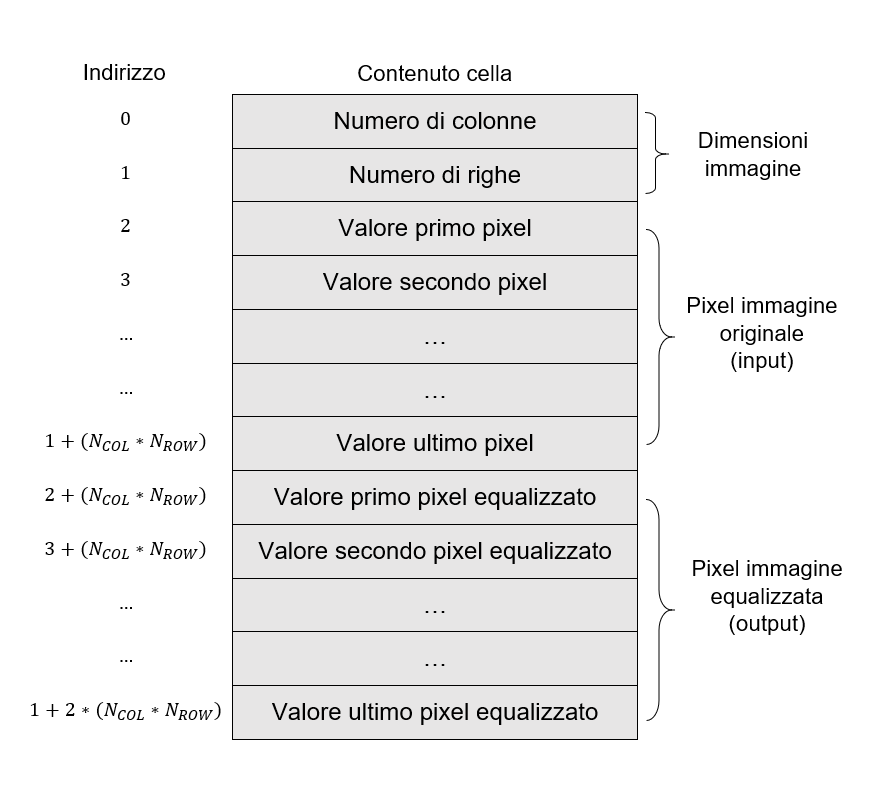
\includegraphics[scale=0.90]{memory_scheme.png}
    \caption{Schema del contenuto delle celle di memoria, con i rispettivi indirizzi}
    \label{fig:memory_scheme}
\end{figure}

\newpage
\subsection{Funzionamento della memoria}
La memoria utilizzata consiste in una Single-Port Block RAM Write-First-Mode.

\bigskip\noindent
La sua interfaccia è la seguente:
\begin{lstlisting}[language=VHDL]
entity rams_sp_wf is
    port(
        clk  : in std_logic;
        we   : in std_logic;
        en   : in std_logic;
        addr : in std_logic_vector(15 downto 0);
        di   : in std_logic_vector(7 downto 0);
        do   : out std_logic_vector(7 downto 0)
    );
end rams_sp_wf;
\end{lstlisting}

\bigskip\noindent
In breve, il funzionamento della memoria richiede che \textbf{en} = 1 per effettuare qualunque operazione (sia lettura che scrittura). 

\bigskip\noindent
A ogni ciclo di clock, viene letto il valore di \textbf{addr}:
\begin{itemize}
    \item se \textbf{we} = 1: viene copiato \textbf{di} nella cella di memoria con indirizzo corrispondente al valore di \textbf{addr}
    \item se \textbf{we} = 0: viene copiato in do il valore contenuto nella cella di memoria con indirizzo corrispondente al valore di \textbf{addr}
\end{itemize}

\bigskip\noindent
In entrambi i casi, tali valori sono disponibili al ciclo di clock successivo.


\newpage
\section{Architettura}
\subsection{Interfaccia del componente}
Il componente implementato presenta la seguente interfaccia:

\begin{lstlisting}[language=VHDL]
entity project_reti_logiche is
    port (
        i_clk     : in std_logic;
        i_rst     : in std_logic;
        i_start   : in std_logic;
        i_data    : in std_logic_vector(7 downto 0);
        o_address : out std_logic_vector(15 downto 0);
        o_done    : out std_logic;
        o_en      : out std_logic;
        o_we      : out std_logic;
        o_data    : out std_logic_vector (7 downto 0)
    );
end project_reti_logiche;
\end{lstlisting}

\begin{itemize}
    \item i\_clk: segnale di CLOCK in ingresso generato dal TestBench
    \item i\_rst: segnale di RESET che inizializza la macchina, in modo che sia pronta per ricevere il primo segnale di START
    \item i\_start: segnale di START generato dal TestBench
    \item i\_data: segnale (vettore) che arriva dalla memoria in seguito a una richiesta di lettura
    \item o\_address: segnale (vettore) di uscita che determina l’indirizzo della memoria su cui effettuare un'operazione
    \item o\_done: segnale di uscita che comunica la fine dell’elaborazione e la completa scrittura del dato in memoria
    \item o\_en: segnale di ENABLE richiesto dalla memoria per poter comunicare, sia in lettura che in scrittura
    \item o\_we: segnale di WRITE ENABLE che deve essere LOW per leggere da memoria e HIGH per scrivere in memoria
    \item o\_data: segnale (vettore) di uscita dal componente verso la memoria
\end{itemize}

\subsection{Scelte progettuali}
Il componente è descritto da due processi:
\begin{itemize}
    \item Il primo rappresenta la parte sequenziale, ossia la gestione dei registri
    \item Il secondo rappresenta la macchina a stati (FSM), che determina lo stato prossimo analizzando lo stato corrente e i segnali in ingresso
\end{itemize}

\subsection{Obiettivi}
Di seguito sono illustrati i principi seguiti durante la progettazione. \\
Notare che, poiché il raggiungimento della massima efficienza non era esplicitamente richiesto, tali principi sono in alcuni caso passati in secondo piano in modo da non compromettere leggibilità e chiarezza sia del codice sorgente che del diagramma degli stati.

\subsubsection{Memoria}
Mantenere in memoria il minor numero di informazioni possibili: ad esempio, soltanto il valore del pixel che sta venendo processato viene salvato.

\subsubsection{Cicli di clock}
Come descritto in precedenza, la memoria rende disponibile il dato richiesto al ciclo di clock successivo. Con l'obiettivo di ridurre al minimo i cicli di clock passati in attesa, quando è necessario un dato la rispettiva richiesta viene, con l'eccezione della lettura di N\_COLUMN e N\_ROW, fatta nello stato precedente.

\subsubsection{Numero di stati} 
Ridurre il più possibile il numero degli stati. In particolare, nelle prime fasi del progetto erano stati previsti più stati per attendere che la memoria rendesse disponibile il dato richiesto. Tali stati sono infine stati collassati nell'unico stato RAM\_SYNC.


\bigskip
\subsection{Descrizione degli stati}
La FSM è composta da 9 stati, come mostrato nel diagramma seguente.
% Immagine diagramma
Di seguito è riportata una breve descrizione di ogni stato:

\subsubsection{IDLE}
Stato iniziale, in cui si attende il segnale di START. \\
Inoltre si ritorna a questo stato quando viene ricevuto il segnale di RESET.
\subsubsection{ASK\_DIM}
Stato in cui viene richiesto alla memoria il numero di colonne dell'immagine (N\_COLUMN), oppure il numero di righe (N\_ROW) in caso in quest'ultimo sia già stato salvato.
\subsubsection{RAM\_SYNC}
In questo stato sono condensate tutte le possibili situazioni di attesa in seguito alla richiesta di un dato alla memoria. \\
Inoltre, esso è in grado di richiedere un dato alla memoria, in modo da minimizzare i cicli di clock passati in attesa.
\subsubsection{READ\_DIM}
In questo stato vengono letti da memoria i valori corrispondenti al numero di colonne e al numero di righe dell'immagine. \\
Inoltre viene calcolato l'indirizzo del primo byte di memoria in cui salvare l'immagine equalizzata, chiamato OUT\_BEGIN
\subsubsection{SAVE\_MAX\_MIN}
Stato in cui viene letta la memoria fino a quando l'indirizzo di lettura non corrisponde a OUT\_BEGIN.
In questo stato vengono salvati il massimo e il minimo valore dei pixel dell'immagine: MAX\_VALUE e MIN\_VALUE
\subsubsection{COMPUTE\_SHIFT}
Stato in cui viene eseguita la prima parte dell'algoritmo di equalizzazione, ossia quella che non dipende da CURRENT\_PIXEL. \\
Viene calcolato DELTA\_VALUE e si ricava SHIFT\_LEVEL discretizzando tramite dei controlli a soglia.
\subsubsection{READ\_PIXEL}
In questo stato viene salvato temporaneamente in memoria il valore del pixel dell'immagine che si sta processando. \\
La lettura dell'immagine procede fino a quando l'indirizzo di lettura non corrisponde a OUT\_BEGIN, in tal caso l'algoritmo è stato completato e il componente passa allo stato DONE.
\subsubsection{EQ\_AND\_WRITE}
In questo stato viene eseguita la seconda parte dell'algoritmo di equalizzazione, ossia quella che dipende da CURRENT\_PIXEL. \\
Vengono calcolati TEMP\_PIXEL e NEW\_PIXEL.
Infine viene richiesta alla memoria la scrittura di NEW\_PIXEl al ciclo di clock successivo.
\subsubsection{DONE}
Stato finale, in cui si attende che il segnale START venga abbassato, per poi tornare nello stato IDLE. 

\newpage
\section{Risultati sperimentali}
\subsection{Report di sintesi}

\subsection{Simulazioni}

\subsubsection{Casi limite}
Per prima cosa sono stati testati i casi limite, usando degli appositi TestBench.
Ne sono stati individuati 5:
\begin{itemize}
    \item Immagine di dimensione 0x0
    \item Immagine di dimensione 1x1
    \item Immagine di dimensione 255x255
    \item Immagine con tutti i pixel a 0
    \item Immagine con tutti i pixel a 255
\end{itemize}

\subsubsection{Risposta ai segnali RESET e START}

\subsubsection{Test generici}
Infine ci si è voluti assicurare del corretto comportamento del componente utilizzando immagini con dimensioni e pixel qualsiasi.

\subsubsection{Pre-sintesi}

\subsubsection{Post-sintesi}

\newpage
\section{Conclusioni}

\end{document}
